This chapter discuss the performance level of a single ipvs load balancer.
(1) Basic functionality and Portability:
We evaluated the load balancer functionality using physical servers in on-premise data center and compared performance level with existing iptables DNAT and nginx as a load balancer.
We also carried out the same performance measurement in GCP and AWS to show the containerized ipvs load balancer is runnable even in the cloud environment.

We will now discuss the feasibility of the proposed load balancer by comparing 
its performance with those of existing iptables DNAT and the Nginx based load balancers. 
We conducted the performance measurements using the benchmark program called wrk\cite{Glozer2016}.

We also investigated the performance varying two network configurations: 
First one is an overlay network setting\cite{Sill2016,Marmol2015} that is often used to build the Kubernetes cluster. 
Flannel\cite{CoreOSFlannel} is one of popular overlay network technologies. 
We compared the performances of three backends settings\cite{CoreOSFlannelBackend}, 
{\it i.e.} operating modes of flannel, to find the best setting.
The other one is the setting for distributed packet processing.
It is well known that distributing handling of interrupts from the network interface card(NIC) 
and the subsequent IP protocol processing, among multiple cores impact the network performance.
In order to derive the best performance from load balancers, 
we also investigated how this setting would affect their performance.

\section{Benchmark method}

The following subsections explain these in further detail. 

\section{Benchmark method}

\begin{figure}
  \centering
  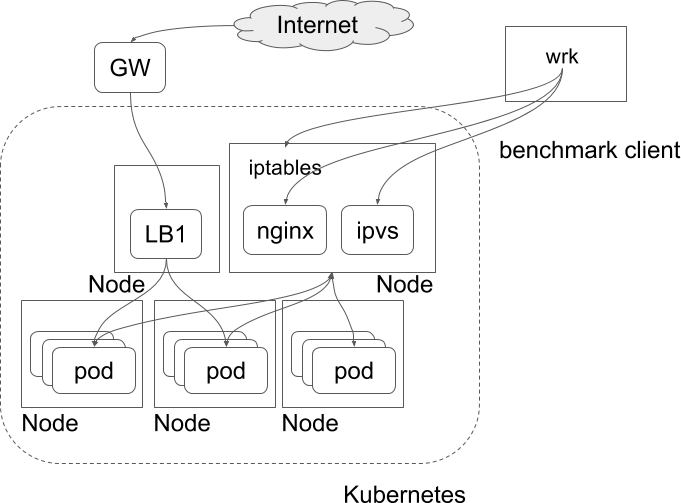
\includegraphics[width=0.8\columnwidth]{Figs/benchmark-schem}
  \caption{Benchmark setup}
  \label{fig:benchmark-schem}
\end{figure}

We measured the performance of the load balancers using the wrk.
Figure~\ref{fig:benchmark-schem} illustrates a schematic diagram of our experimental setup.
Multiple {\em pods} are deployed on multiple nodes in the Kubernetes cluster. 
In each {\em pod}, a Nginx web server that returns the IP address of the {\em pod} are running.
We then set up the IPVS, iptables DNAT, and Nginx load balancers on one of the nodes(the top right node in the Figure~\ref{fig:benchmark-schem}). 

We measured the throughput, Request/sec, of the web service running on the Kubernetes cluster as follows:
The HTTP GET requests are sent out by the wrk on the client machine toward the nodes,
using destination IP addresses and port numbers that are chosen based on the type of the load balancer on which the measurement is performed.
The load balancer on the node then distributes the requests to the {\em pods}.
Each {\em pod} will return HTTP responses to the load balancer, after which the load balancer returns them to the client.
Based on the number of responses received by wrk on the client, 
load balancer performance, in terms of Request/sec can be obtained. 

Figure~\ref{fig:benchmark example} shows an example of the command-line for wrk and the corresponding output.
The command-line in Figure~\ref{fig:benchmark example} will generate 40 wrk program threads 
and allow those threads to send out a total of 800 concurrent HTTP requests over the period of 30 seconds.
The output example shows information including per thread statistics, error counts, Request/sec and Transfer/sec.

Figure~\ref{fig:Hardware and software configuration} shows hardware and software configuration used in our experiments.
We configured Nginx HTTP server to return a small HTTP content, 
the IP address of the {\em pod}, to make a relatively severe condition for load balancers. 
The size of the character string making up an IP address is limited to 15 bytes.
If we had chosen the HTTP response size so that most of the IP packet resulted in maximum transmission unit(MTU), 
the performance would have been limited by the Ethernet bandwidth.
However, since we used small HTTP responses, we could purely measure the load balancer performance.

The hardware we used had eight physical CPU cores and a NIC with 4 rx-queues.


\begin{figure}[t]
  \centering
  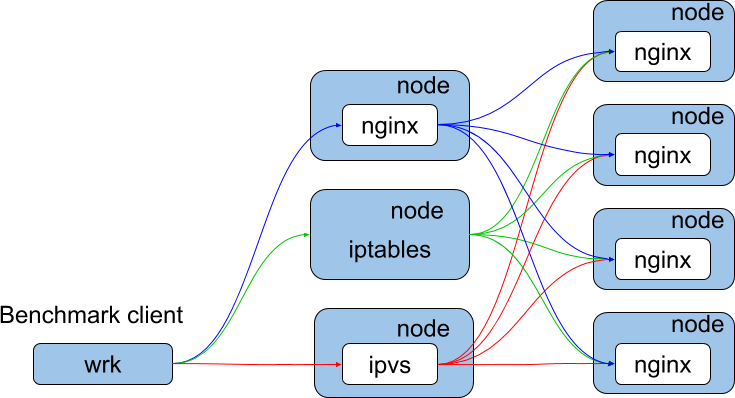
\includegraphics[width=0.7\columnwidth]{Figs/lb_single_schem}
  \caption{}
  \label{fig:lb_single_schem}
\end{figure}

\begin{table}[]
  \centering
  \begin{tabular}{l}
    \hline
    \begin{minipage}{12cm}
      \begin{verbatim}

[Command line] 
 wrk -c800 -t40 -d30s http://172.16.72.2:8888/ 
-c: concurrency, -t: # of thread, -d: duration 

[Output example] 
 Running 30s test @ http://10.254.0.10:81/ 
  40 threads and 800 connections 
  Thread Stats   Avg      Stdev     Max   +/- Stdev 
    Latency    15.82ms   41.45ms   1.90s    91.90\% 
    Req/Sec     4.14k   342.26     6.45k    69.24\% 
  4958000 requests in 30.10s, 1.14GB read 
  Socket errors: connect 0, read 0, write 0, timeout 1 
Requests/sec: 164717.63 
Transfer/sec:     38.86MB 
      \end{verbatim}
    \end{minipage}
   \\ \hline
  \end{tabular}
  \caption{}
  \label{tab:bench_example}
\end{table}

\begin{table}[]
  \centering
  \begin{tabular}{ll}
    \hline \\
    \multicolumn{2}{l}{[Hardware Specification]}   \\
    & CPU: Xeon E5-2450 2.10GHz x 8 (with Hyper Threading) \\
    & Memory: 32GB \\
    & NIC: Broadcom BCM5720 Giga bit \\
    & (Node x 6, LB x 1, Client x 1) \\
    & \\
    \multicolumn{2}{l}{[Node Software]}  \\
    & OS: Debian 8.7, linux-3.16.0-4-amd64 \\
    & Kubernetes v1.10.6 \\
    & flannel v0.7.0 \\
    & etcd version: 3.0.15 \\
    & \\
    \multicolumn{2}{l}{[Container Software]}   \\
    & Keepalived: v1.3.2 (12/03,2016) \\
    & nginx : 1.11.1(load balancer), 1.13.0(web server) \\
    \\ \hline
  \end{tabular}
  \caption{}
  \label{tab:hw_sw_spec}
\end{table}


Throughput measurements were carried out in order to examine the basic functionality of the containerized ipvs load balancer.
Fig.~\ref{fig:benchmark-schem} shows the schematic diagram of the throughput measurement and summarizes experimental conditions.
We measured the performance of the load balancers using a benchmark program called wrk\cite{Glozer2016}.
Multiple nginx {\em pods} are deployed on multiple nodes as web servers in the Kubernetes cluster.
In each nginx {\em pod}, single nginx web server that returns the IP address of the {\em pod} is running.
We then set up the ipvs, iptables DNAT, and nginx load balancers on one of the nodes, and performed the throughput measurement.
The throughput is measured by sending out HTTP requests from the wrk towards a load balancer and by counting the number of responses the benchmark host received as shown in Fig.~\ref{fig:benchmark-schem}~(\subref{fig:lb_single_schem}).

Fig.~\ref{fig:benchmark-schem}~(\subref{fig:bench_example}) shows an example of the command-line for wrk and the corresponding output.
The command-line in Fig.~\ref{fig:benchmark-schem}~(\subref{fig:bench_example}) will generate 40 wrk program threads
and allow those threads to send out a total of 800 concurrent HTTP requests over the period of 30 seconds.
The output example shows information including per-thread statistics, error counts, throughput in [Request/sec] and data rate in [Transfer/sec]

Fig.~\ref{fig:benchmark-schem}~(\subref{fig:hw_sw_spec}) shows hardware and software configuration used in our experiments.
We used a total of eight servers; six servers for Nodes, one for the load balancer and one for the benchmark client, with all having the same hardware specifications.
The software versions used for Kubernetes, web server and load balancer {\em pods} are also summarized in the figure.


\section{Results}

\begin{figure}
  \centering
  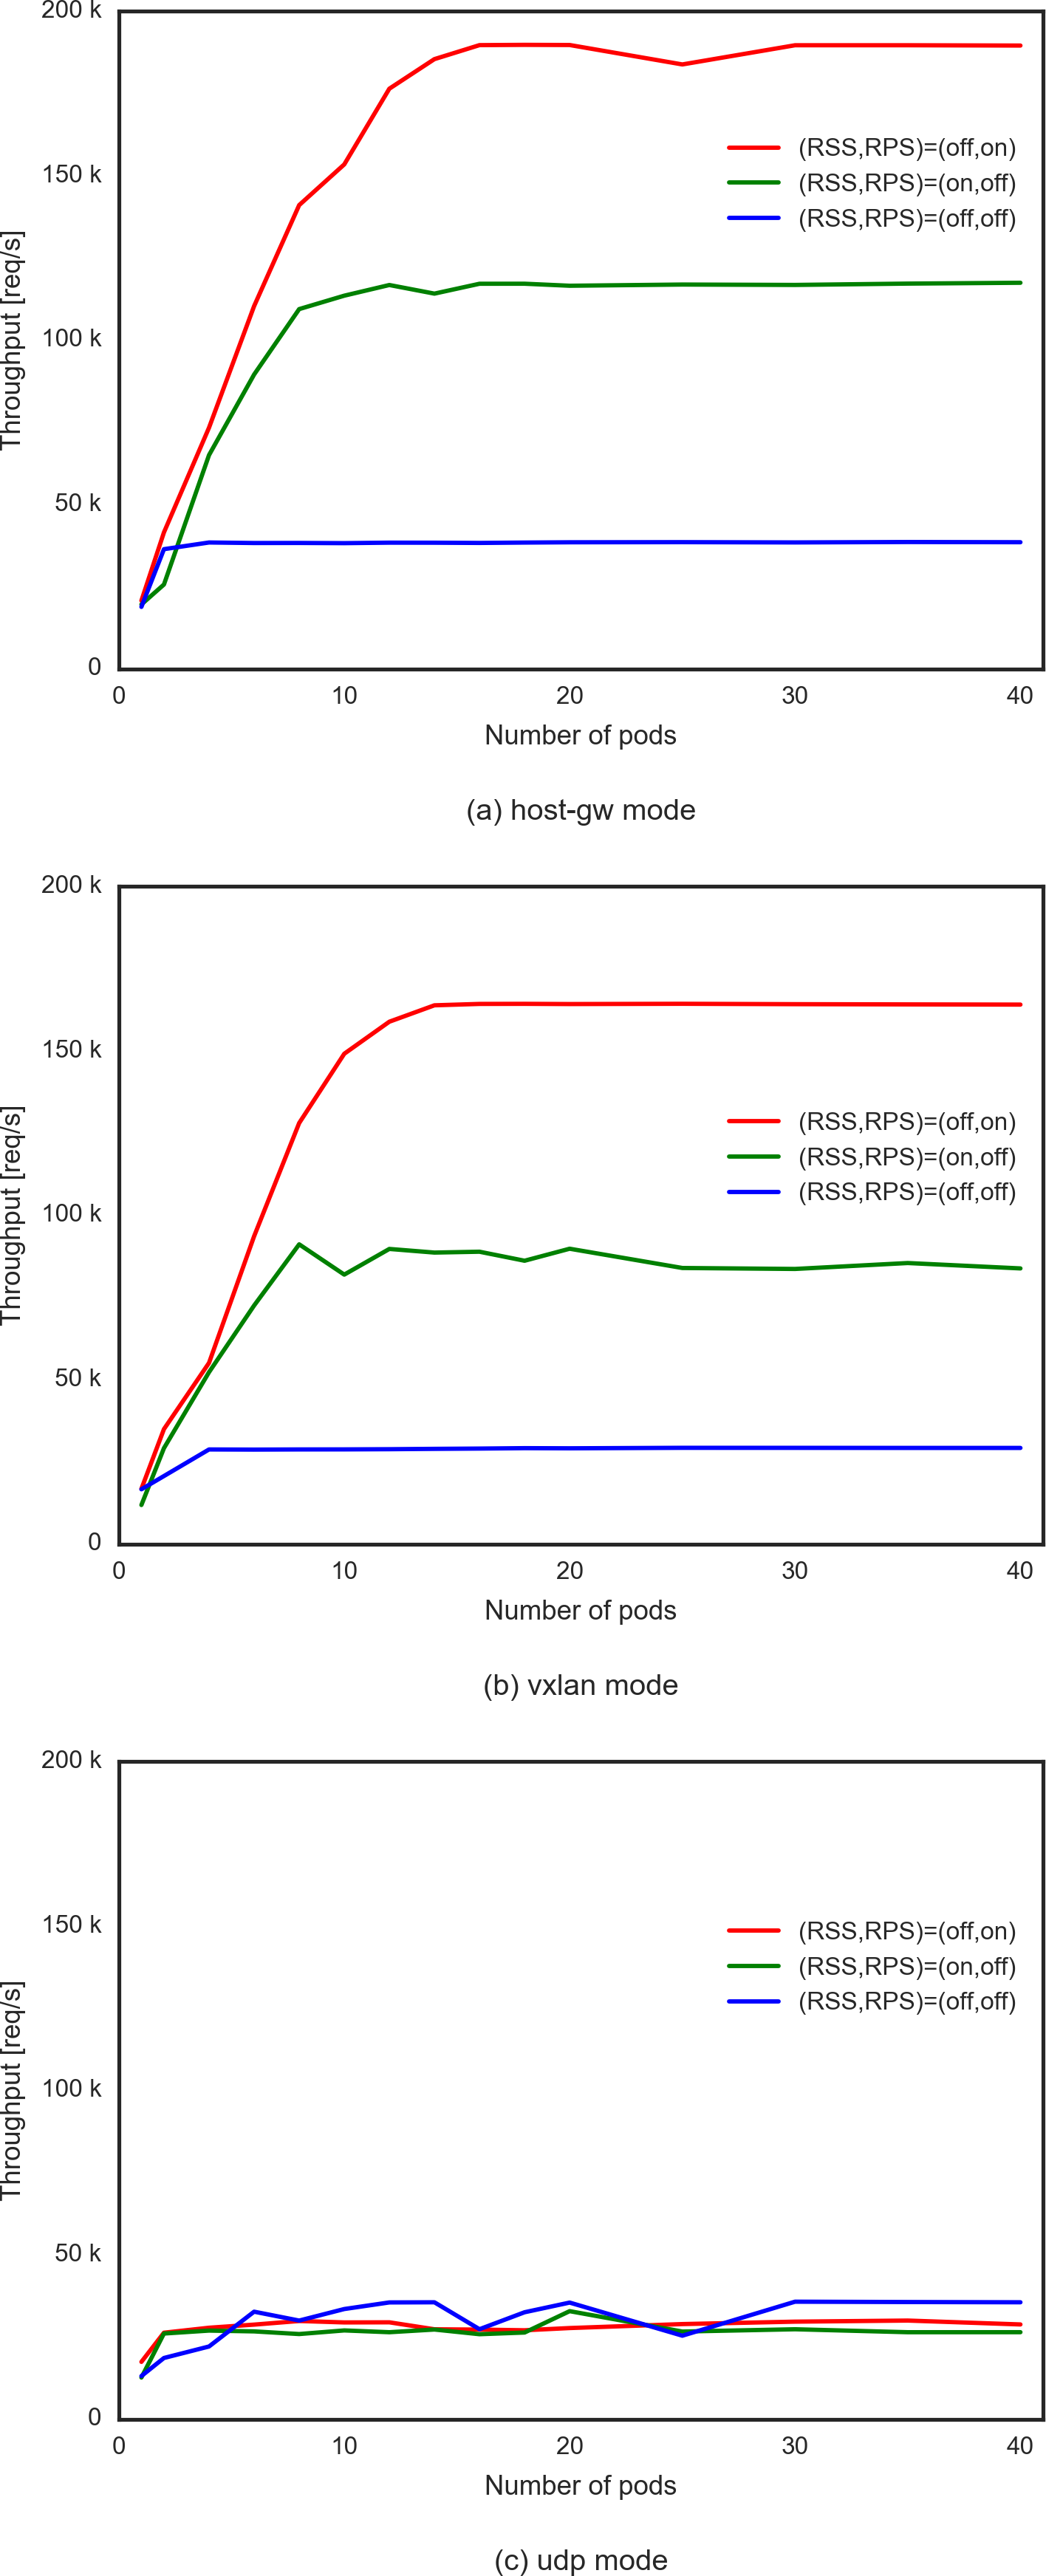
\includegraphics[width=0.6\columnwidth]{Figs/ipvs_3figs}
  \caption{IPVS results}
  \label{fig:IPVS3figs}
\end{figure}

\begin{figure}
  \centering
  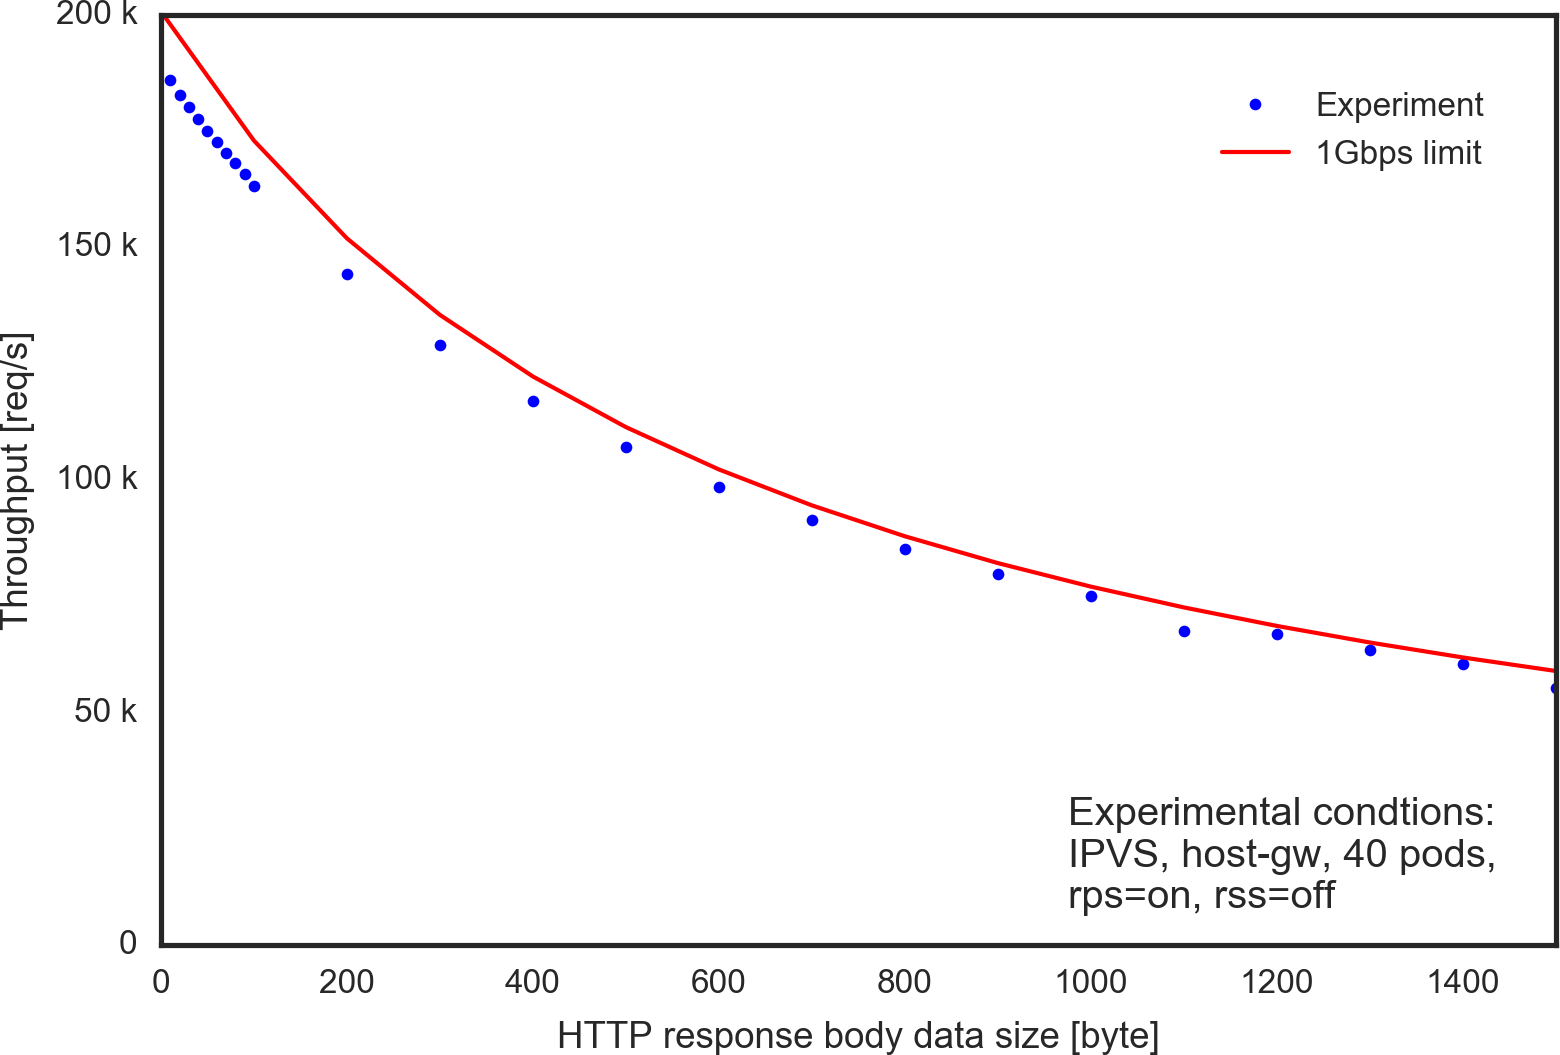
\includegraphics[width=0.8\columnwidth]{Figs/performance_limitation}
  \caption{Performance limitation due to 1Gbps bandwidth}
  \label{fig:performance_limitation}
\end{figure}

\begin{figure}
  \centering
  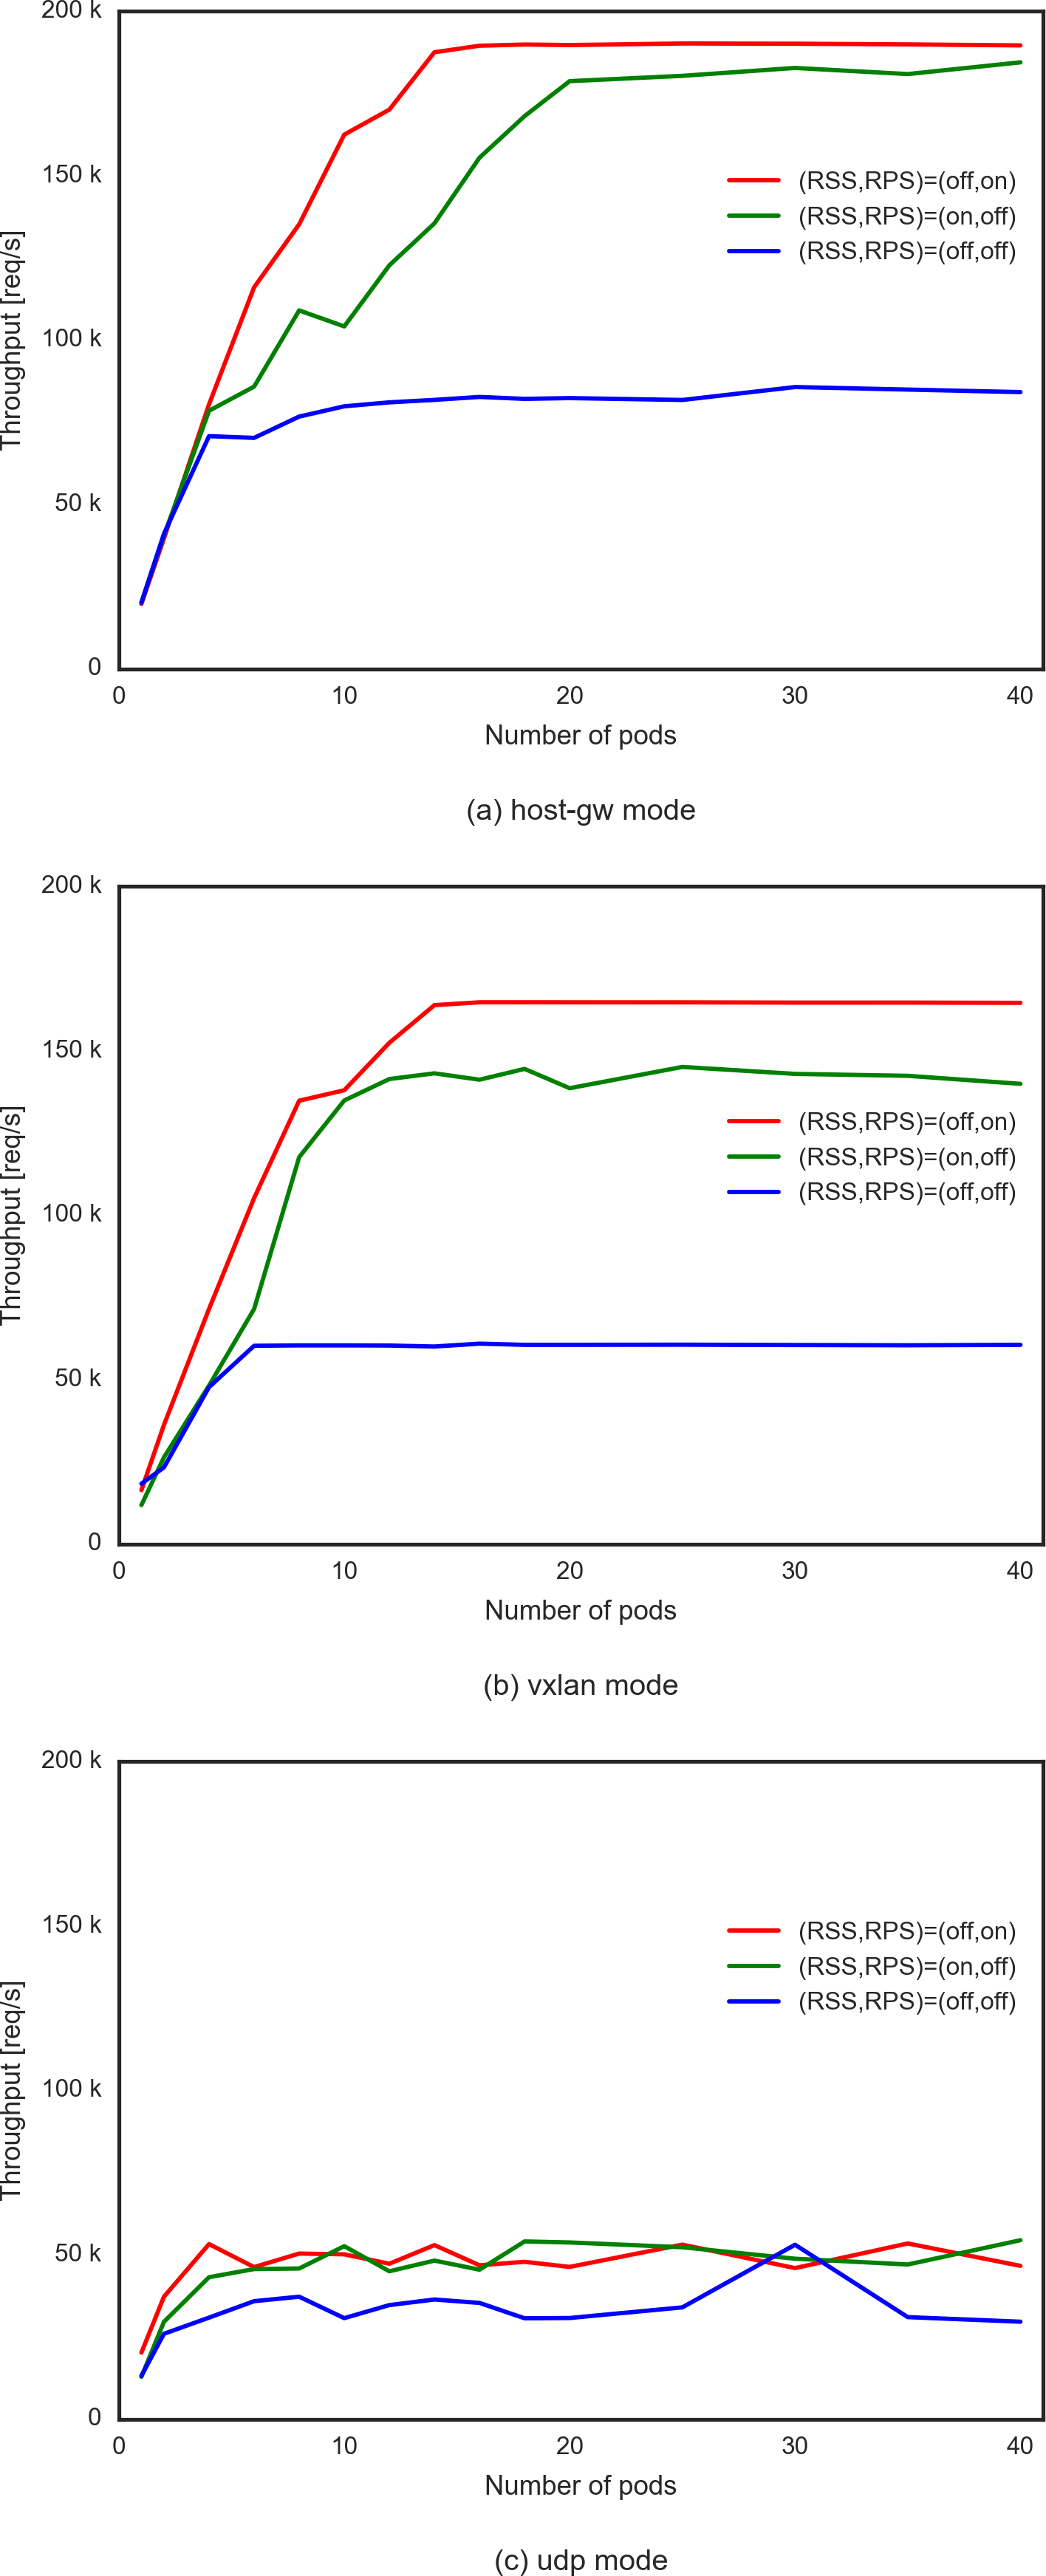
\includegraphics[width=0.6\columnwidth]{Figs/iptables_3figs}
  \caption{iptables results}
  \label{fig:iptabls3figs}
\end{figure}

\begin{figure}
  \centering
  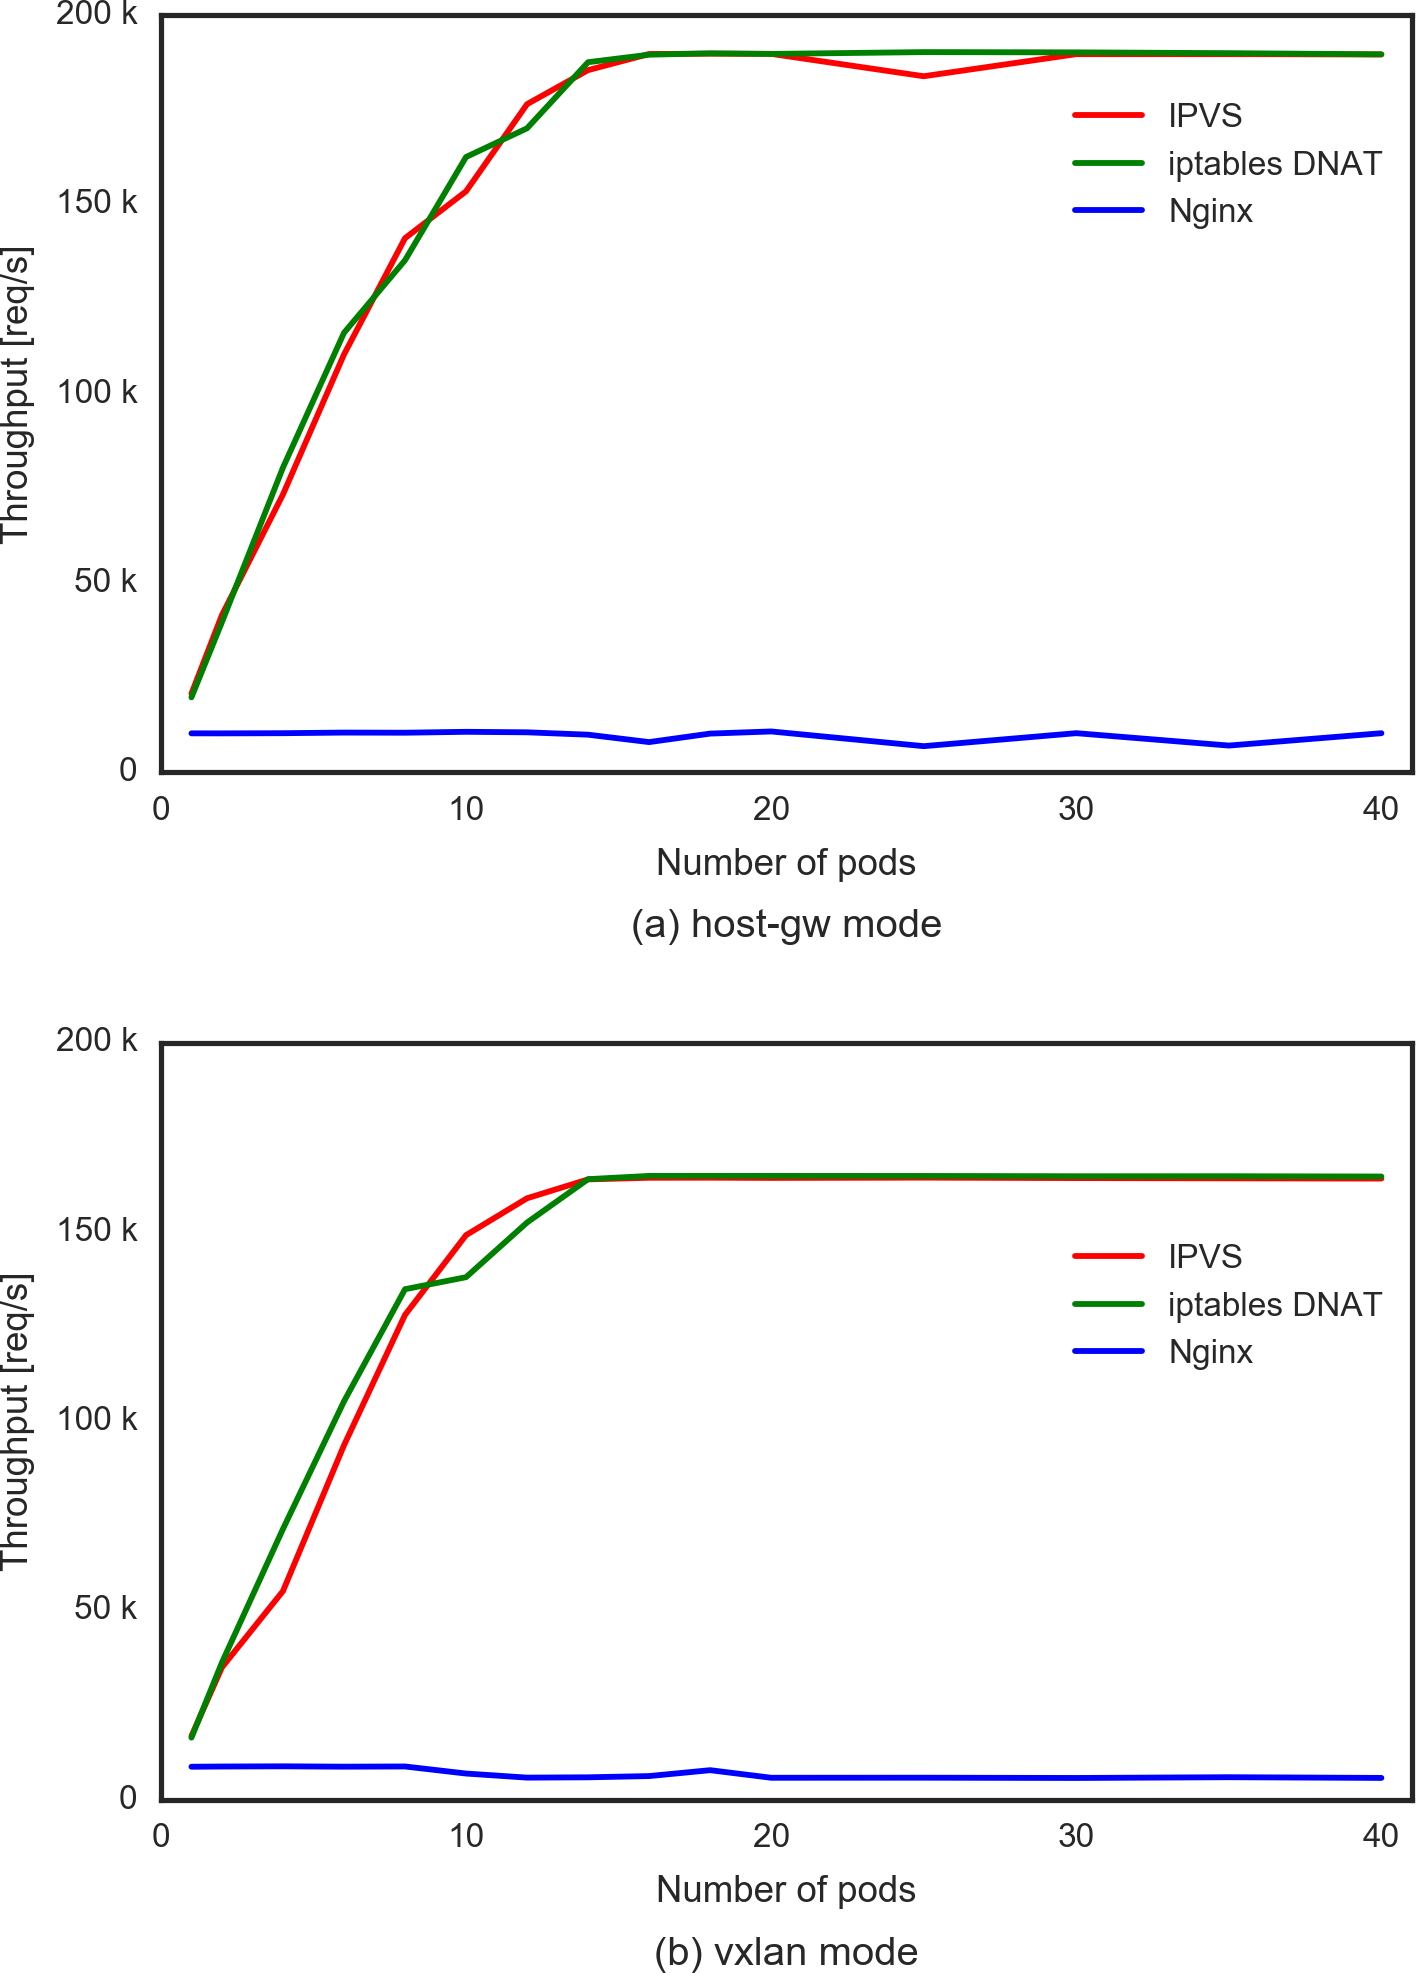
\includegraphics[width=0.8\columnwidth]{Figs/ipvs-iptables-nginx_2figs}
  \caption{IPVS and iptables comparison}
  \label{fig:IPVS-iptables-nginx_2figs}
\end{figure}

\begin{figure}
  \centering
  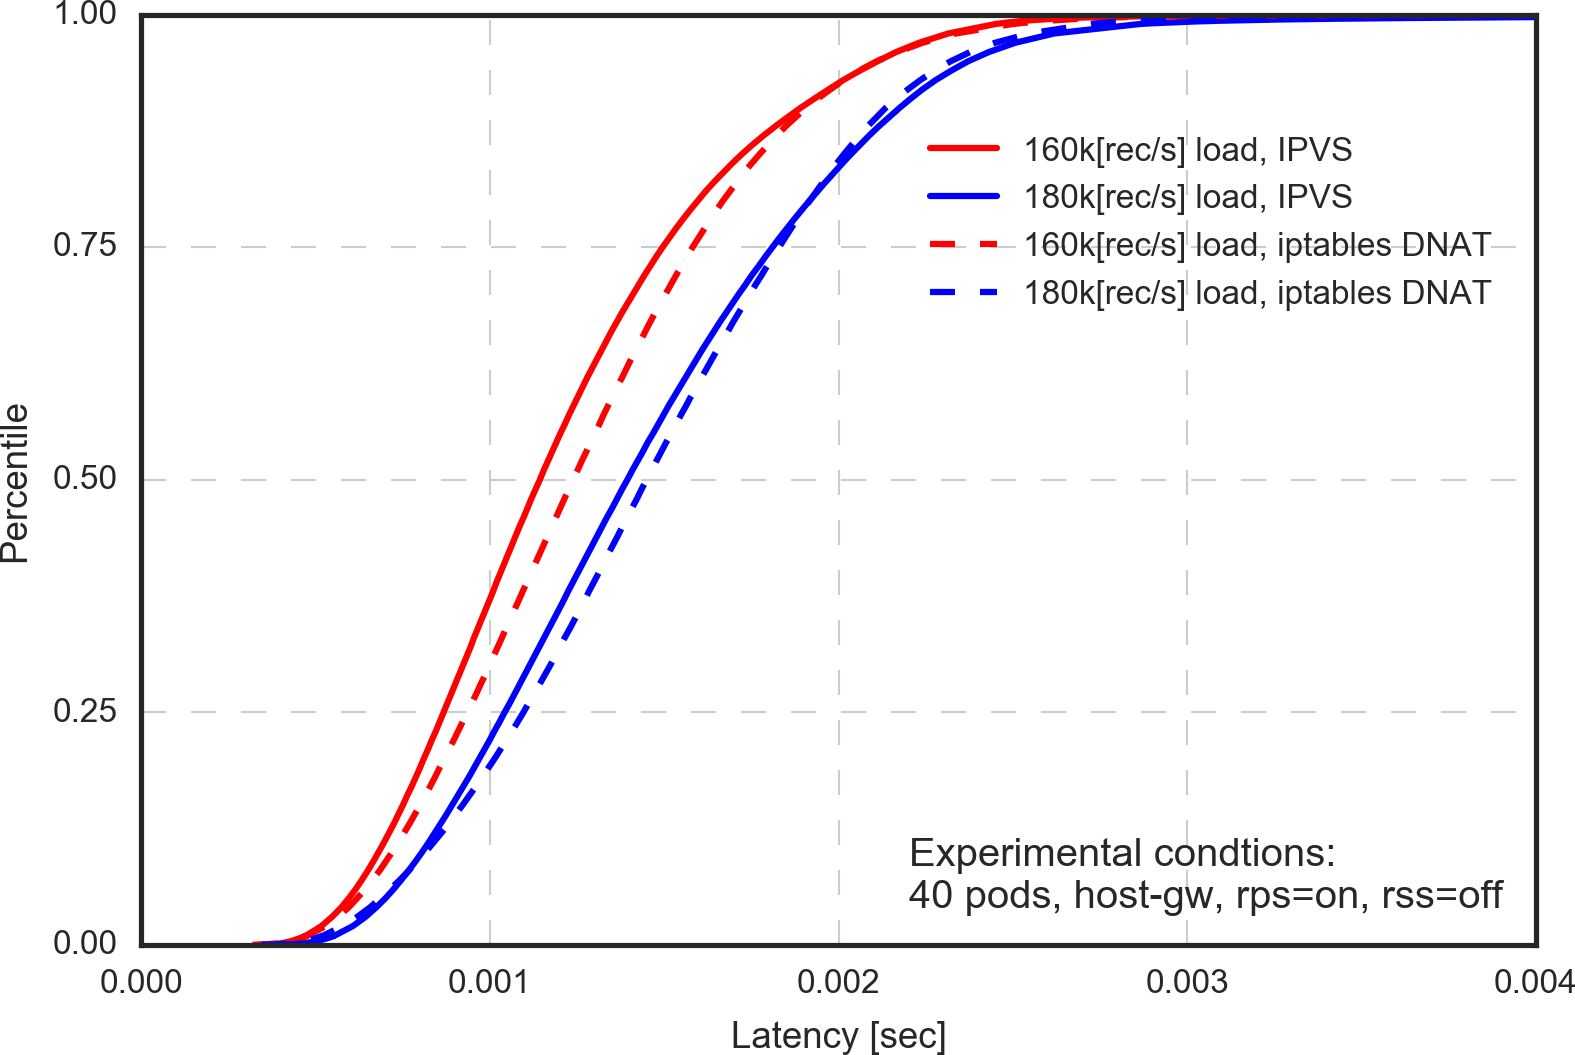
\includegraphics[width=0.8\columnwidth]{Figs/latency_cdf_rps_40pods}
  \caption{Latency cumulative distribution function}
  \label{fig:latency_cdf_rps_40pods}
\end{figure}


Figure~\ref{fig:IPVS3figs} shows the IPVS load balancer performance, that is, 
the throughput (Request/sec) of the Nginx web server {\em pods} in our experiments.
As for the overlay network, we measured the performance for three flannel backend modes, 
host-gw (Figure~\ref{fig:IPVS3figs}(a)), vxlan (Figure~\ref{fig:IPVS3figs}(b)) and udp (Figure~\ref{fig:IPVS3figs}(c)).
The following RSS and RPS setting were compared: 

\begin{center}
  \centering
  \begin{minipage}{0.8\columnwidth}
\begin{verbatim}
(RSS, RPS) = (off, off)
           = (on , off)
           = (off, on )
\end{verbatim}
  \end{minipage}
\end{center}

Except for the udp cases, we can see the trend in which the throughput linearly increases 
as the {\em pod} number increases and then it eventually saturates.
The saturated performance levels indicates the maximum performance of the IPVS load balancer.
The maximum performance limits depend on the flannel backend mode type and the (RSS, RPS) settings.
From the results in Figures~\ref{fig:IPVS3figs}(a,b), it can be seen that if we turn off distributed packet processing,
{\it i.e.}, when \enquote{(RSS, RPS) = (off, off)}, performance degrades significantly. 
In this case, the performance bottleneck is primarily due to packet processing in a single core.

If we compare the results for the cases when \enquote{(RSS, RPS) = (on, off)} and \enquote{(RSS, RPS) = (off, on)},
the latter is better than the former.
This is understandable, since in the case of \enquote{RPS = on}, eight physical cores can be used whereas 
in the case of \enquote{RSS = on} only four cores can be used, on the hardware used in our experiment.
The performance bottleneck of the case when \enquote{RSS = on} is considered 
to be due to the fact that the packet processing is only done on four CPU cores.
%
At first, it was not clear what caused the performance limit for the case when \enquote{RPS = on},
however we now suspect this is due to 1Gbps bandwidth limitation.
A packet level analysis using tcpdump\cite{jacobson1989tcpdump} revealed that 622.72 byte of extra HTTP headers, 
TCP/IP headers and ethernet frames are needed for each request in the case of the wrk benchmack program.  
This results in the upper limitation of 196,627 [req/s], where the date size of HTTP response body is 13 byte, or typical data size in our experiment. 
Figure~\ref{fig:performance_limitation} shows upper limitation of the performance level for 1Gbps ethernet together with 
actual benchmark results and we can conclude that when \enquote{RPS = on}, IPVS performance is limited by bandwidth.

If we compare the performances among the flannel backend modes types, 
the host-gw mode where no encapsulation is conducted shows the highest performance level,
followed by the vxlan mode where the Linux kernel encapsulate the Ethernet frame.
The udp mode where flanneld itself encapsulate the IP packet shows significantly lower performances levels.

Figure~\ref{fig:iptabls3figs} shows the performance of the load balancer 
functionality of the iptables DNAT. 
As can be seen in the figure, the performance value increases as the number of the {\em pod} increases linearly, 
and then becomes saturated at some point, as was the case with the IPVS results.

If we compare the results for different packet handling settings, the highest performance is 
obtained for the case when \enquote{(RSS, RPS) = (off on)}, followed by the case when \enquote{(RSS, RPS) = (on, off)}. 
The performance result for the case when \enquote{(RSS, RPS) = (off, off)} resulted in the 
poorest performance level, as was the case for the IPVS.
As for the flannel backend modes, the host-gw shows the highest performance followed 
by the vxlan. The udp backend mode totally degrades the performance level.

Figure~\ref{fig:IPVS-iptables-nginx_2figs} compares the performance measurement results 
among the IPVS, iptables DNAT, and Nginx load balancers
with the condition of \enquote{(RSS, RPS) = (off on)}.
The proposed IPVS load balancer exhibits almost equivalent performance as the existing iptables DNAT based load balancer. 
The Nginx based load balancer shows no performance improvement even though the number of the Nginx web server {\em pods} is increased.
It is understandable because the performance of the Nginx as a load balancer is expected to be similar to the performance as a web server.
Figure~\ref{fig:latency_cdf_rps_40pods} compares Cumulative Distribution Function(CDF) of the load balancer latency at the constant load.
The latencies are a little bit smaller for IPVS, however we consider the difference almost negligible.
For example, the median value at 160K[req/s] load for IPVS and iptables DNAT are, 1.1 msec and 1.2 msec, respectively.
So, we can conclude our proposed load balancer showed no performance degradation while providing potability.

\section{Basic functionality and portability}


\begin{figure}[t]
  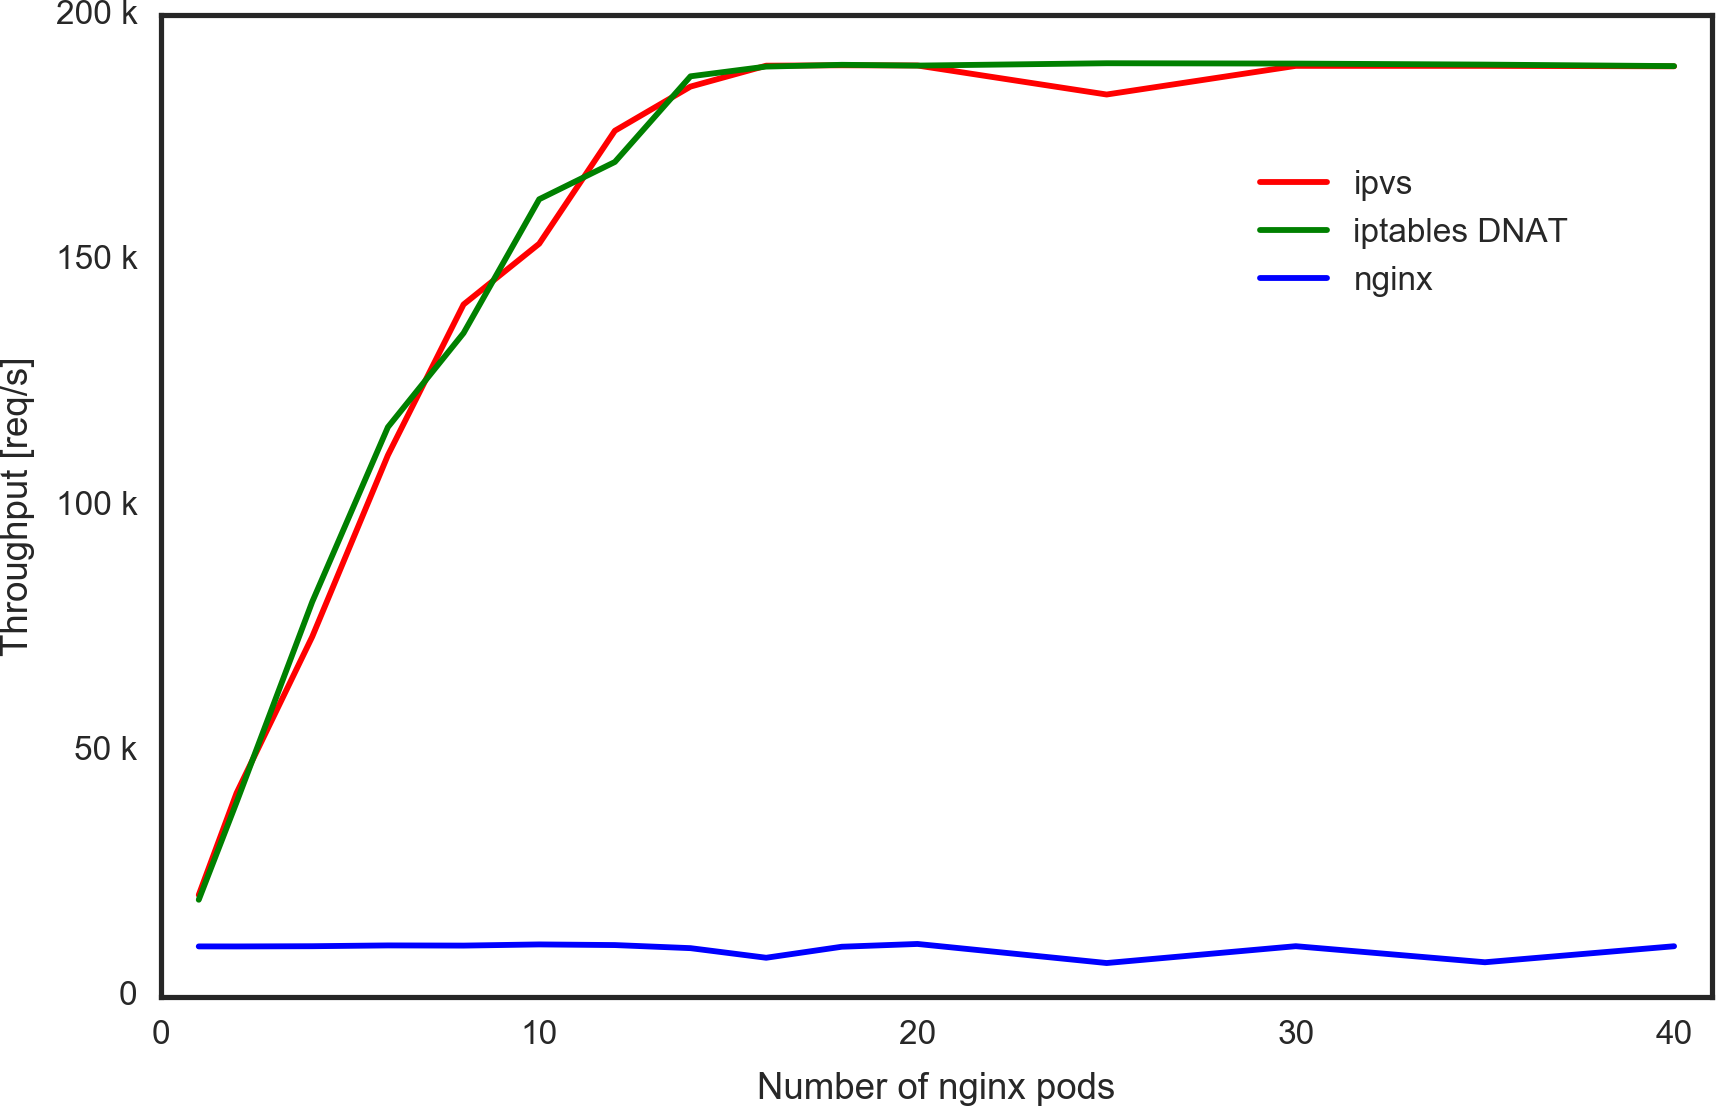
\includegraphics[width=0.9\columnwidth]{Figs/ipvs-iptables-nginx}
  \caption{Performance of the load balancer container.}
  \label{fig:ipvs-iptables-nginx}
\end{figure}


\begin{figure}[t]
    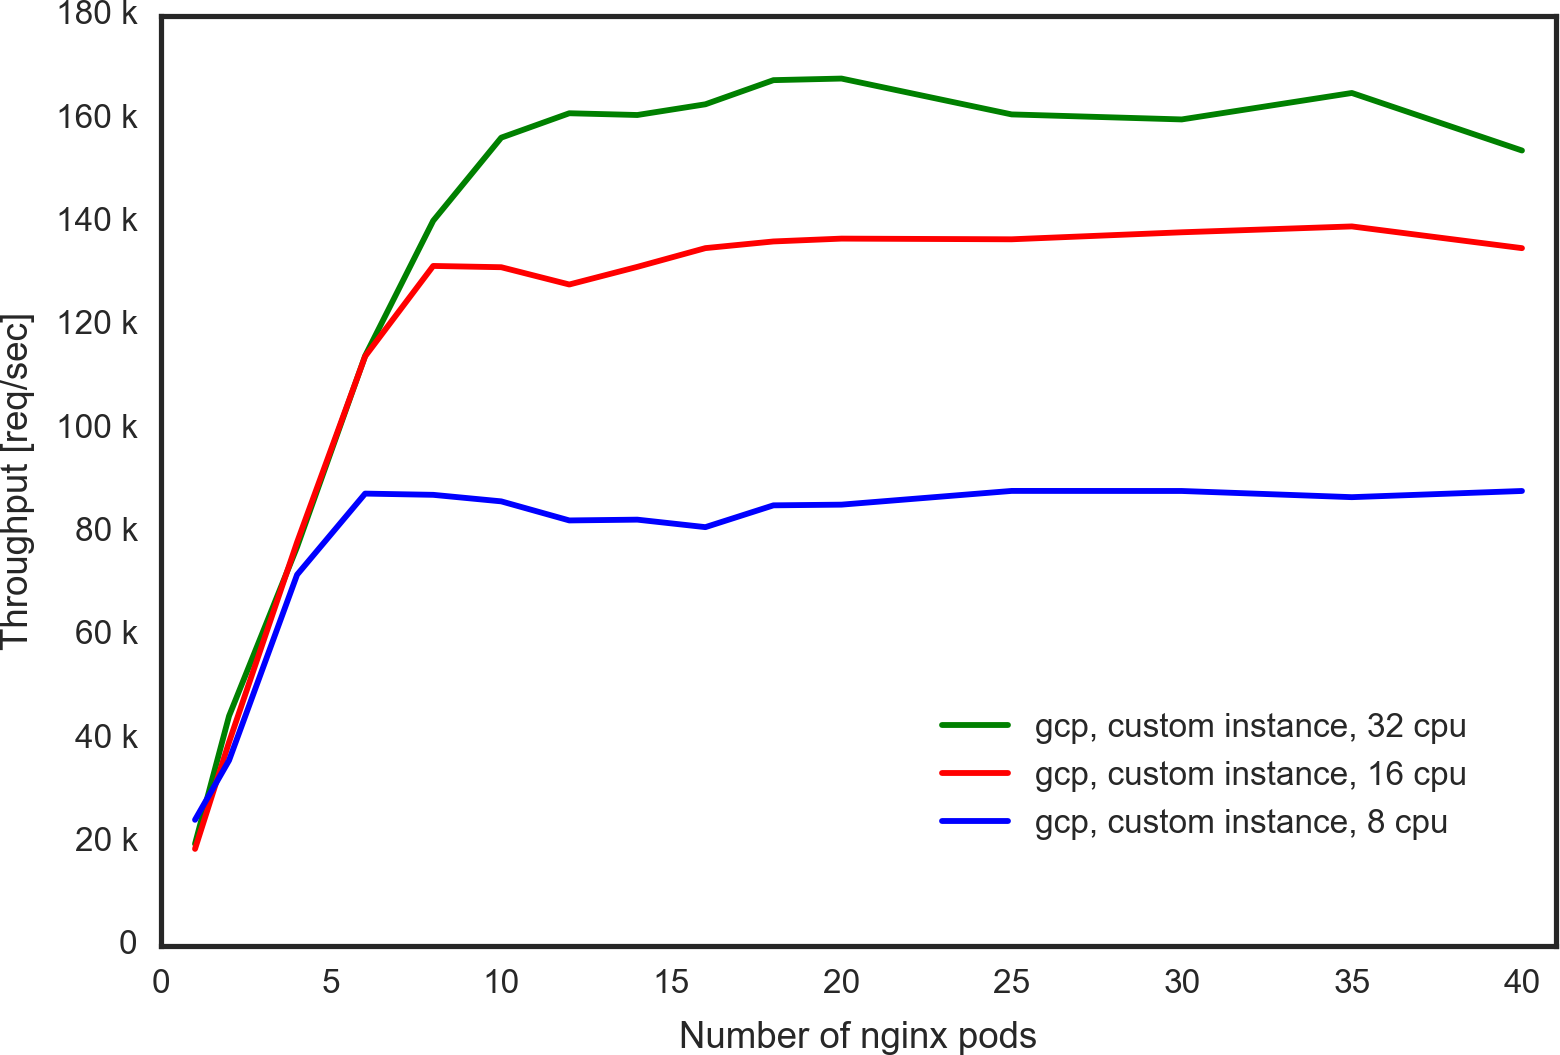
\includegraphics[width=0.9\columnwidth]{Figs/gcp_all_ieice}
    \caption{GCP}
    \label{fig:gcp_all_ieice}
\end{figure}

\begin{figure}[t]
    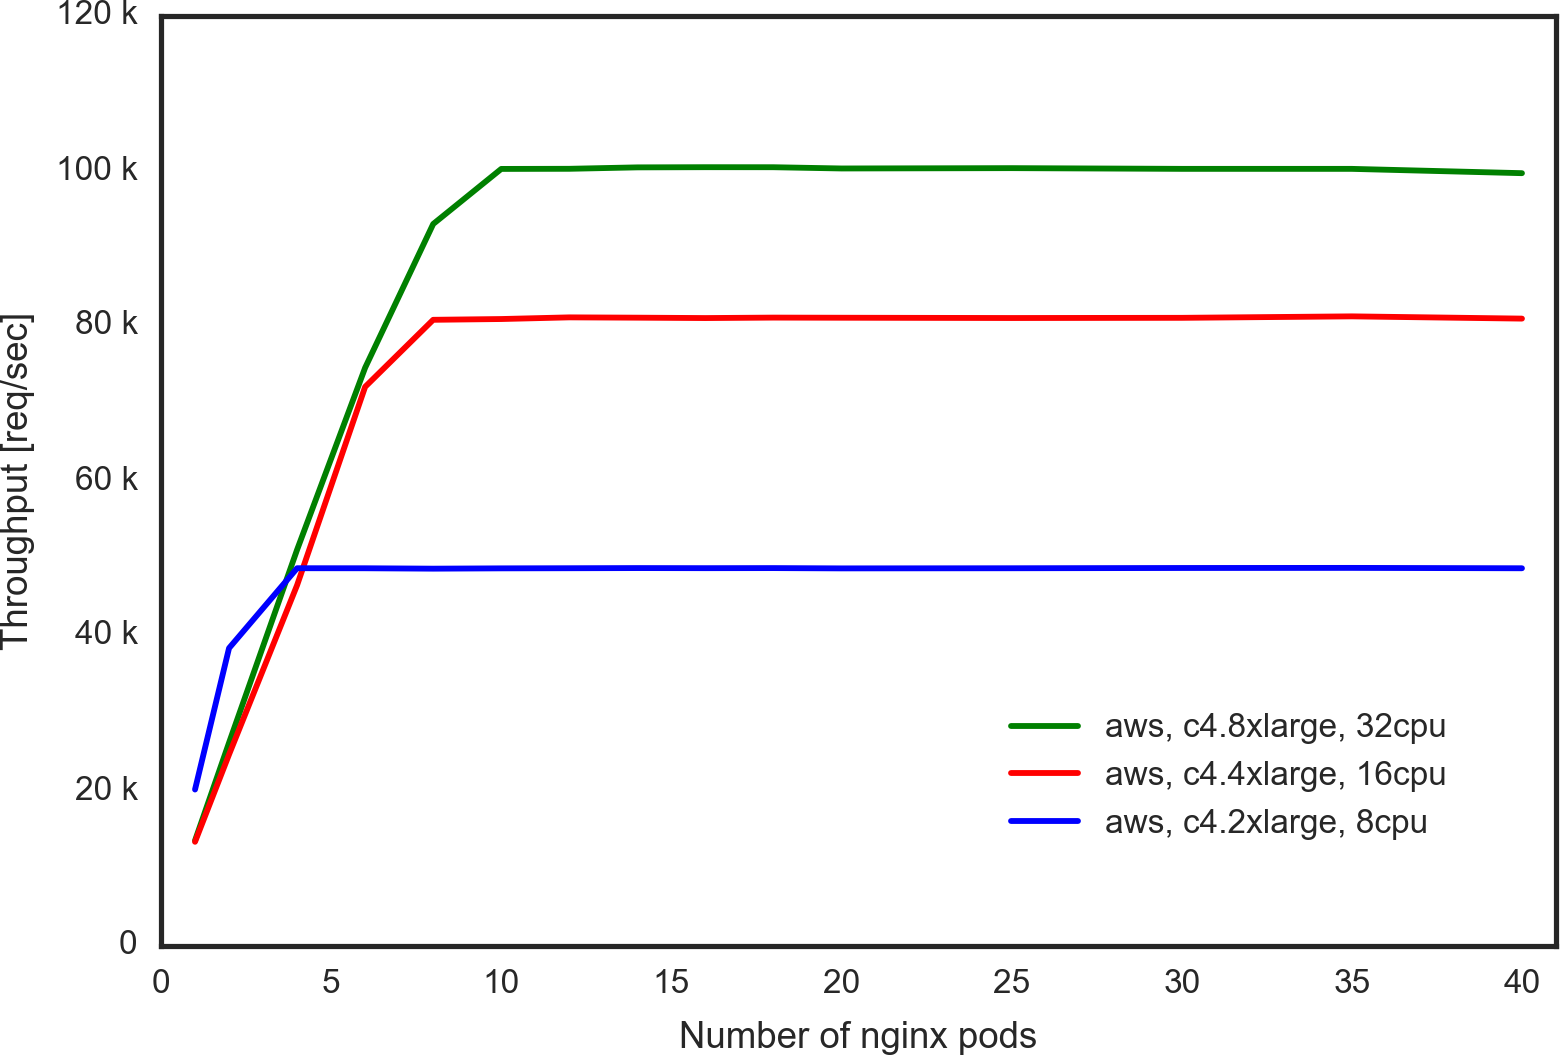
\includegraphics[width=0.9\columnwidth]{Figs/aws_c4_ieice}
    \caption{AWS with Node x 6, Client x 1, Load balancer x 1. Custom instance. }
    \label{fig:aws_c4_ieice}
\end{figure}

%\interfootnotelinepenalty=10000

Fig.~\ref{fig:ipvs_performance}~(\subref{fig:ipvs-iptables-nginx}) shows the throughput of the proposed ipvs container load balancer.
The performance of the nginx and the iptables DNAT as the load balancers are also presented for comparison.
As we increased the number of the nginx pods(web servers) from 1 to around 14, the throughput increased almost linearly and after which it saturated.
The increase indicates that the load balancer functions properly because it increased throughput by distributing HTTP requests to multiple of the web servers.
The saturated performance level indicates the maximum performance of the load balancer, which could be determined either by network bandwidth or CPU level of the load balancer or the benchmark client.
In this specific experiment, the performance level was limited by the 1 Gbps bandwidth of experimental network\cite{takahashi2018portable}, which is revealed by packet level analysis using tcpdump.\footnote{
On average the data size of each request was about 636 [byte/req] including TCP/IP headers, ethernet header, and interframe gaps.
Multiplying that with 190K [req/sec] and 8 [bit/byte] will result in 966.72 Mbps.
}
While nginx did not show any benefit as the load balancer, the performance of the ipvs load balancer container showed equivalent performance level as the un-containerized iptables DNAT.
This means that our proposed ipvs container load balancer is at least as good as the un-containerized iptables' load balancing in the 1 Gbps network.

Fig.~\ref{fig:ipvs_performance}~(\subref{fig:gcp_all_ieice}) and Fig.~\ref{fig:ipvs_performance}~(\subref{fig:aws_c4_ieice}) show the load balancer performance levels that are measured in GCP and AWS, respectively.
These are aimed to show that our proposed load balancer can be run in cloud environments and also functions properly.

Both results show similar characteristics as the experiment in an on-premise data center in Fig.~\ref{fig:ipvs_performance}~(\subref{fig:ipvs-iptables-nginx}), where throughput increased linearly to a certain saturation level that is determined by either network speed or machine specifications.
Since in the cases of cloud environments we can easily change the machine specifications, especially CPU counts, we measured throughput with several conditions of them.
From the first look of the results, since changing CPU counts changed the load balancer's throughput saturation levels, we thought VM's computation power limited the performance levels.
However, since there are cases in the cloud environment, where changing the VM types or CPU counts also changes the network bandwidth limit, a detailed analysis is further required in the future to clarify which factor limits the throughput in the cases of these cloud environments.
Still, we can say that the proposed ipvs load balancers can be run in GCP and AWS, and function properly until they reach the infrastructure limitations.

\section{Resource Consumption}

\section{Summary}



